\section{Preliminary}
\label{sec:prelim}

\subsection{Notation and Formalization}

In this paper, we study budgeted capability distillation from a large teacher model \(T\) to a
smaller student model \(S\), with total training-token budget \(B\). Let
\(\mathcal{C}=\{c_1,\ldots,c_{|\mathcal{C}|}\}\) denote a set of measurable
capabilities\rev{, here the eight core capabilities of Appendix Table~\ref{tab:capabilities-benchmarks},} and let \(s_k(M)\) be model \(M\)'s benchmark score on capability
\(c_k\). A distillation strategy \(\pi\) specifies how data is generated, how
the teacher is queried, and how tokens are allocated across capabilities,
assigning budgets \(\{b_k\}\) with \(\sum_k b_k\le B\), and producing a
distilled student \(S_\pi\).

\begin{definition}[Capability distillation]\label{def:cap_distill}
Given a teacher model \( T \), an initial student model \( S_0 \), and
capability-specific data distributions \( \{ \mathcal{D}_c \}_{c\in\mathcal{C}} \),
capability distillation allocates a limited budget \( B \) across capabilities
to improve task-relevant performance under shared representations by optimizing
a weighted mixture of distillation objectives:
\begin{equation}
\begin{aligned}
\min_{S,\,\mathbf{w}} \;&
\mathbb{E}_{x\sim \mathcal{D}_{\mathbf{w}}}
\!\left[\ell\!\left(S(x),T(x)\right)\right] \quad\
\text{s.t.} \quad\
\mathbf{w}\in\Delta_{|\mathcal{C}|},\; \mathrm{cost}(S;S_0)\le B .
\end{aligned}
\end{equation}
where \( \mathcal{D}_{\mathbf{w}} := \sum_{c\in\mathcal{C}} w_c \mathcal{D}_c \), and $\mathrm{cost}(S;S_0)$ measures the distillation token budget consumed to obtain $S$ from $S_0$.
Here \( \mathbf{w}=(w_c)_{c\in\mathcal{C}} \) lies in the probability simplex
\rev{\( \Delta_{|\mathcal{C}|}=\{\mathbf{w}\in\mathbb{R}^{|\mathcal{C}|} \mid w_c\ge 0,\ \sum_{c\in\mathcal{C}} w_c=1\} \)},
which specifies the allocation of training effort across capabilities, and
\( \ell \) denotes a standard distillation loss, such as token-level
cross-entropy or logit-matching between the student\rev{'s and the teacher's output distributions}.
\end{definition}

\rev{Under shared representations, budget spent on one capability changes the
others. We measure this cross-capability effect by distilling with one-hot allocations:}
\begin{definition}[Capability interdependence]\label{def:cap_interdependence}
Let \( S_0 \) be an initial student model, and let \( S(\mathbf{w},B) \) denote
the student obtained after capability distillation under allocation
\( \mathbf{w}\in\Delta_{|\mathcal{C}|} \) and budget \( B \). For each capability
\( c_i \), define the one-hot allocation vector
\( \mathbf{w}^{(i)}\in\Delta_{|\mathcal{C}|} \) by \( w^{(i)}_i=1 \) and
\( w^{(i)}_j=0 \) for all \( j\neq i \). The \emph{capability interdependence}
under capability distillation is characterized by the capability transfer matrix
\[
\mathbf{T}_{ij}(B)
:= s_j\!\left(S(\mathbf{w}^{(i)},B)\right) - s_j(S_0),
\]
where $\mathbf{T}(B)\in\mathbb{R}^{|\mathcal{C}|\times|\mathcal{C}|}$, \( \mathbf{T}_{ij}(B) \) quantifies the effect of distilling
toward capability \( c_i \) on the performance of capability \( c_j \).
Non-zero off-diagonal entries indicate interdependence between capabilities
under shared representations.
\end{definition}

\vspace{-0.6em}
\subsection{Exploratory Study and Problem Formulation}
\label{sec:emp_res}

\rev{We distill Llama-3.3-70B-Instruct into Llama-3.1-8B-Instruct under fixed
token budgets, one target capability at a time, and evaluate the student on all
benchmarks to form the transfer matrix of Definition~\ref{def:cap_interdependence}
(strategies and settings in Appendix~\ref{sec:app_em}). All
benchmark metrics are accuracies or success rates on a $0$--$100$ scale, a
capability score is the unweighted mean over its benchmarks, and every entry of
the transfer matrix is an absolute difference in these points
(Definition~\ref{def:cap_interdependence}); no further rescaling is applied
(Appendix~\ref{sec:app_em}).}

%==================== Figure 1: empirical study (top float; all four panels share one height) ====================
\begin{figure}[t]
  \centering
  \captionsetup[sub]{font=footnotesize,skip=2pt}
  % capability legend as a single row: the two rows of icon.pdf, cropped and placed side by side
  
\includegraphics[height=11pt,trim=0 232 50 43,clip]{figure/icon.pdf}\hspace{0.8em}%
  
\includegraphics[height=11pt,trim=0 0 50 275,clip]{figure/icon.pdf}\\[3pt]
  % panel widths follow from a common height of 72pt and each PDF's aspect ratio
  \begin{subfigure}[b]{0.181\linewidth}
    \centering
    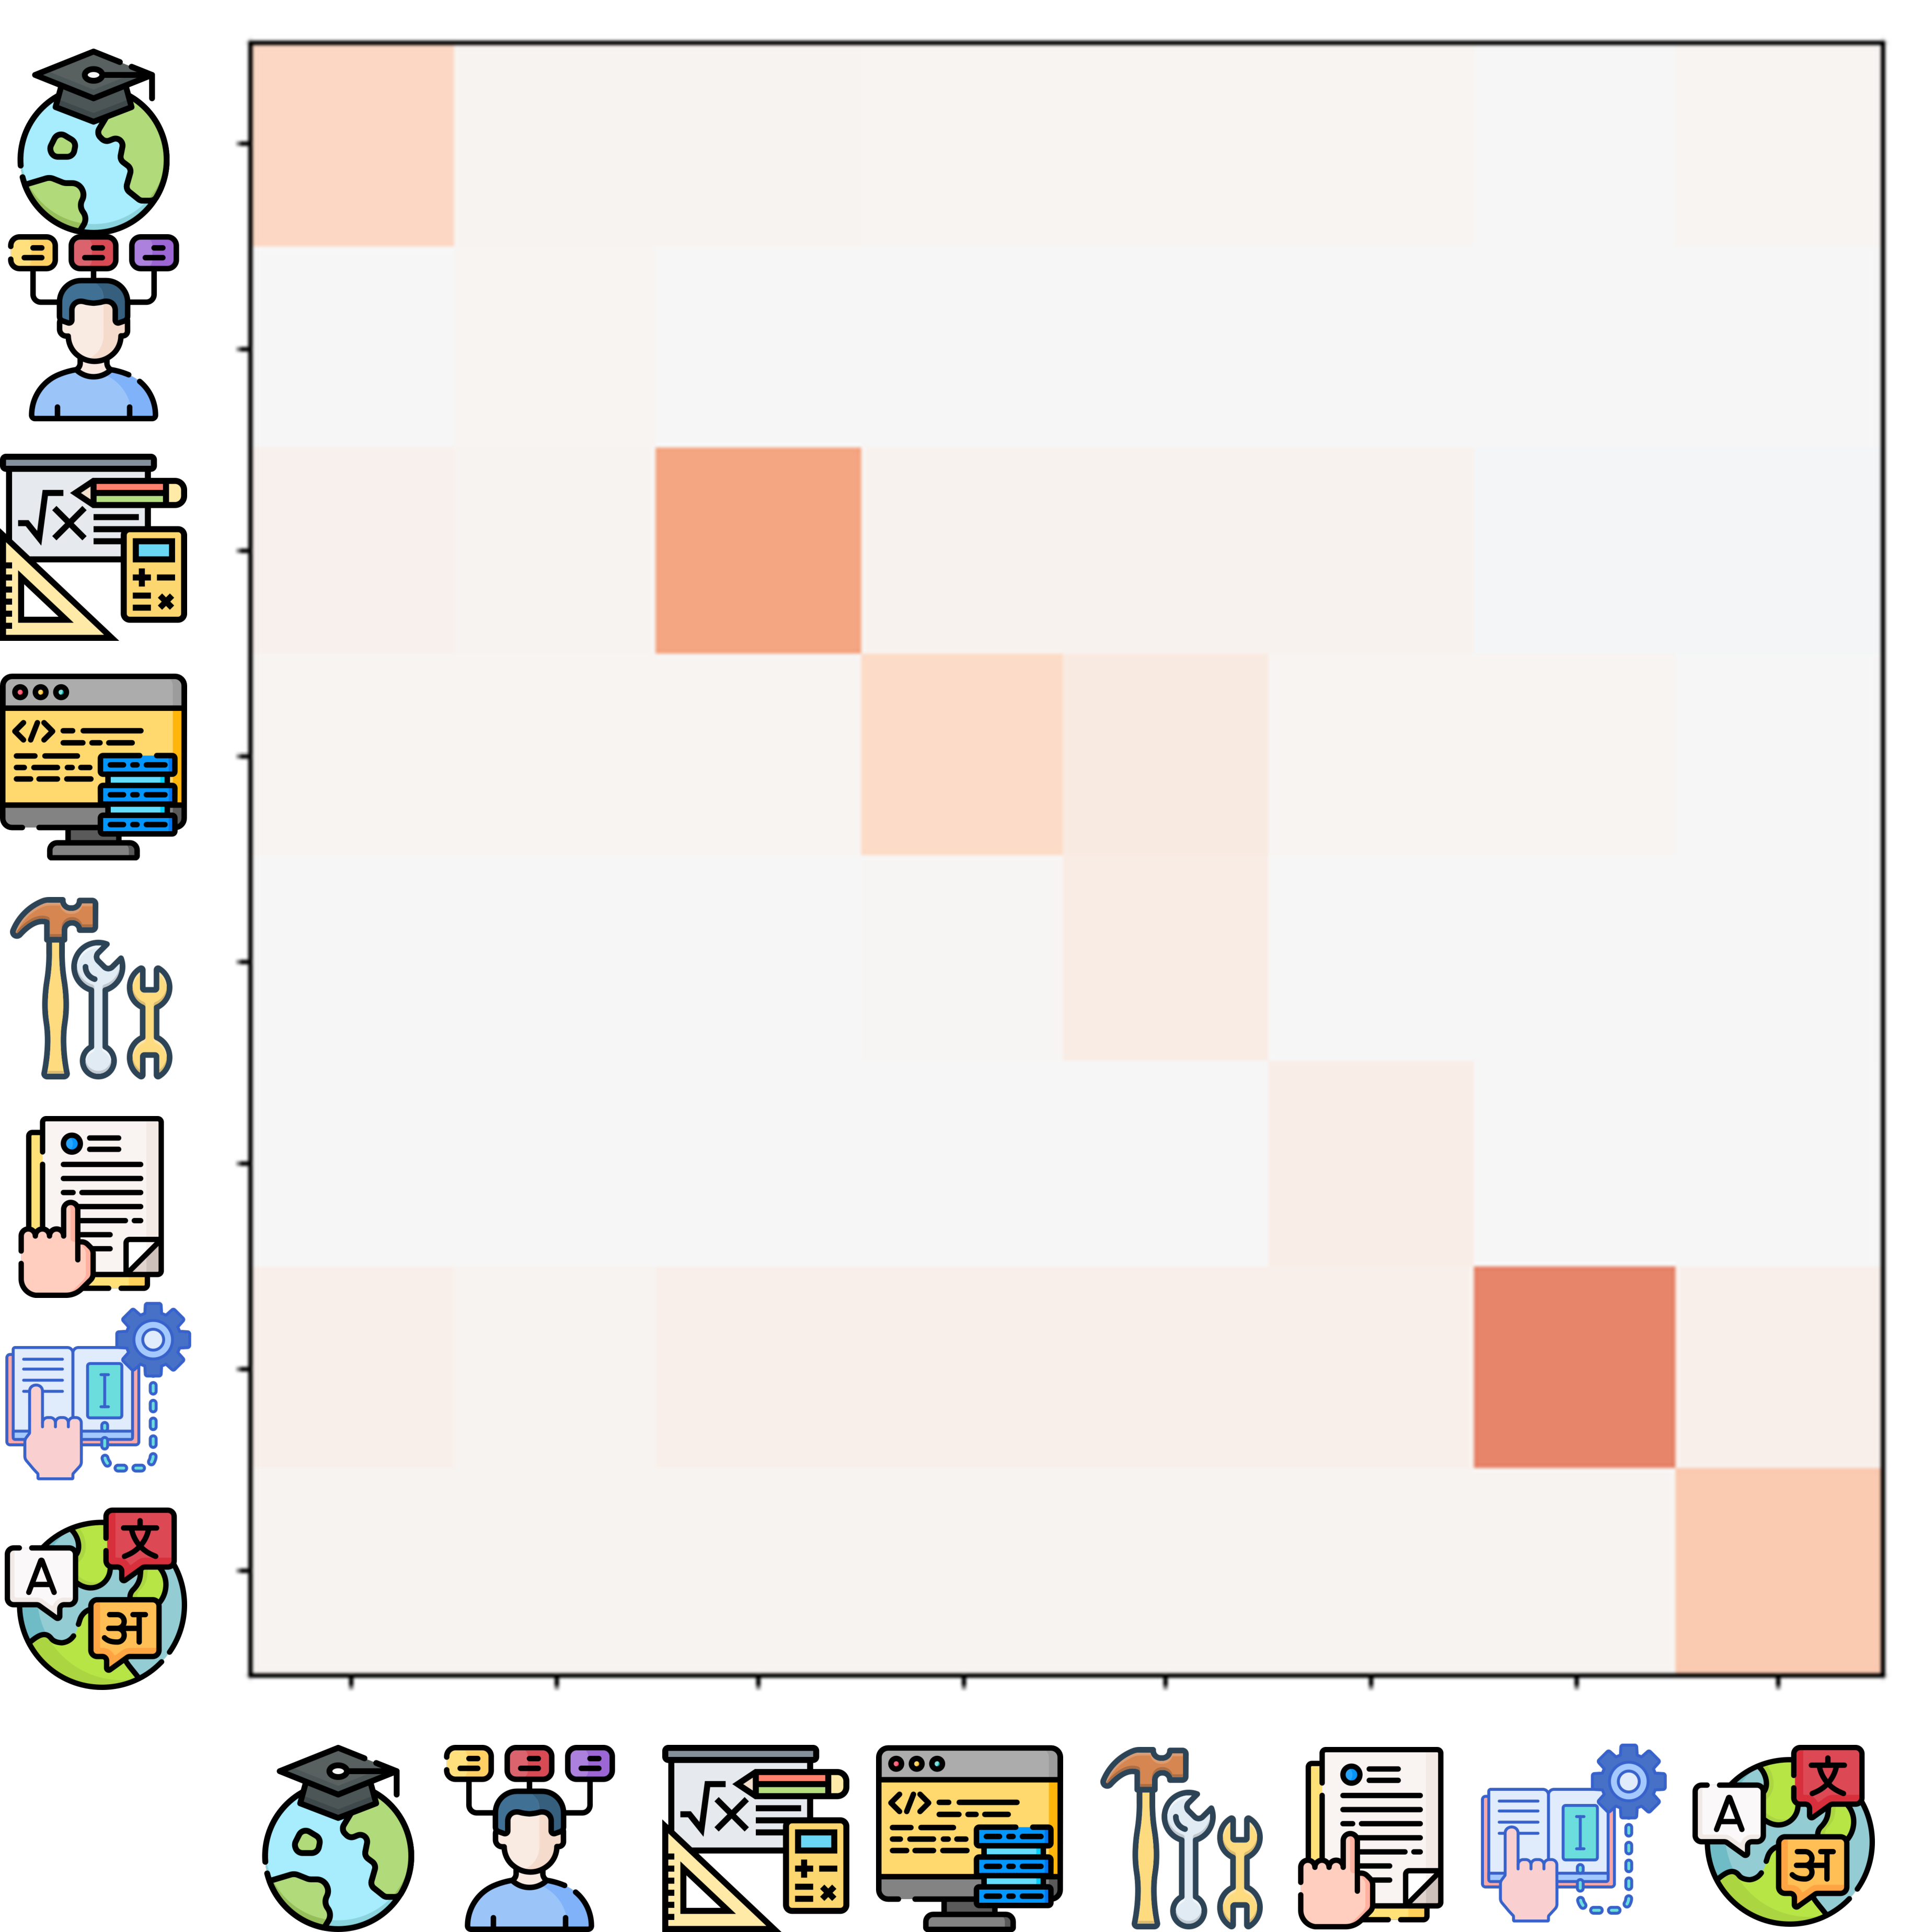
\includegraphics[height=72pt]{figure/heatmap_small.pdf}
    \caption{Small budget}
    \label{fig:heatmap_small}
  \end{subfigure}\hfill
  \begin{subfigure}[b]{0.209\linewidth}
    \centering
    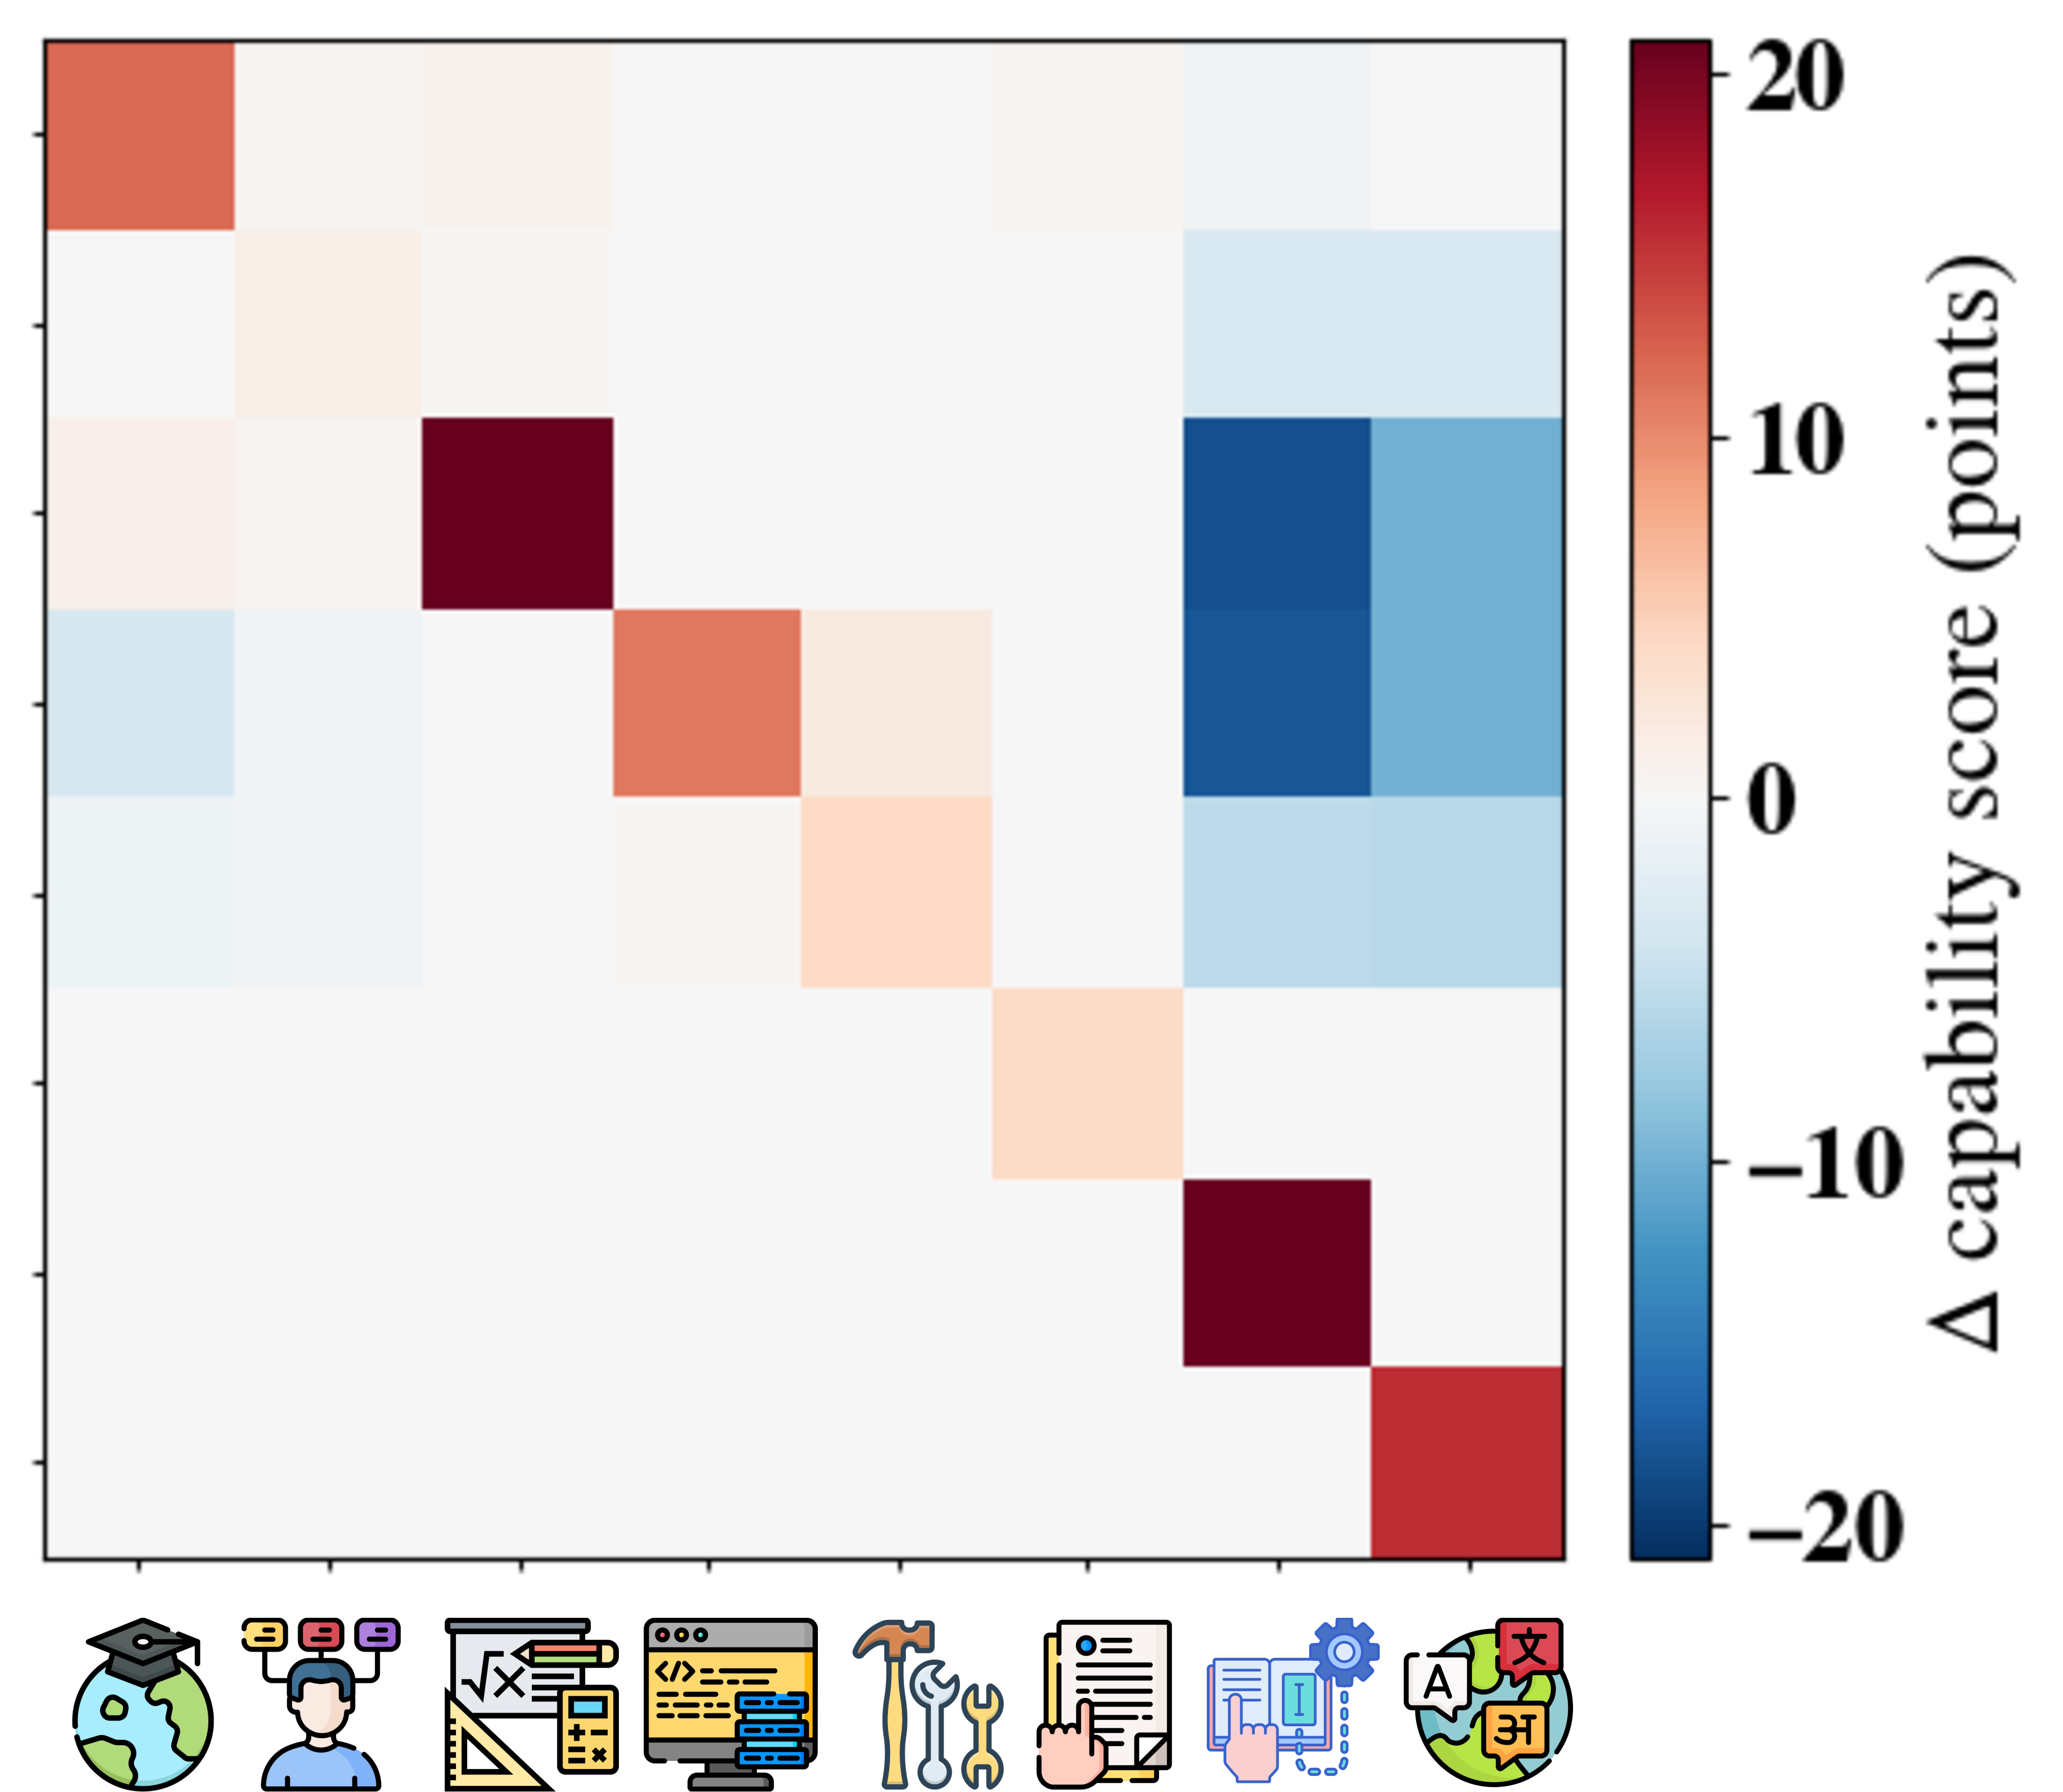
\includegraphics[height=72pt]{figure/heatmap_large.pdf}
    \caption{Large budget}
    \label{fig:heatmap_large}
  \end{subfigure}\hfill
  \begin{subfigure}[b]{0.306\linewidth}
    \centering
    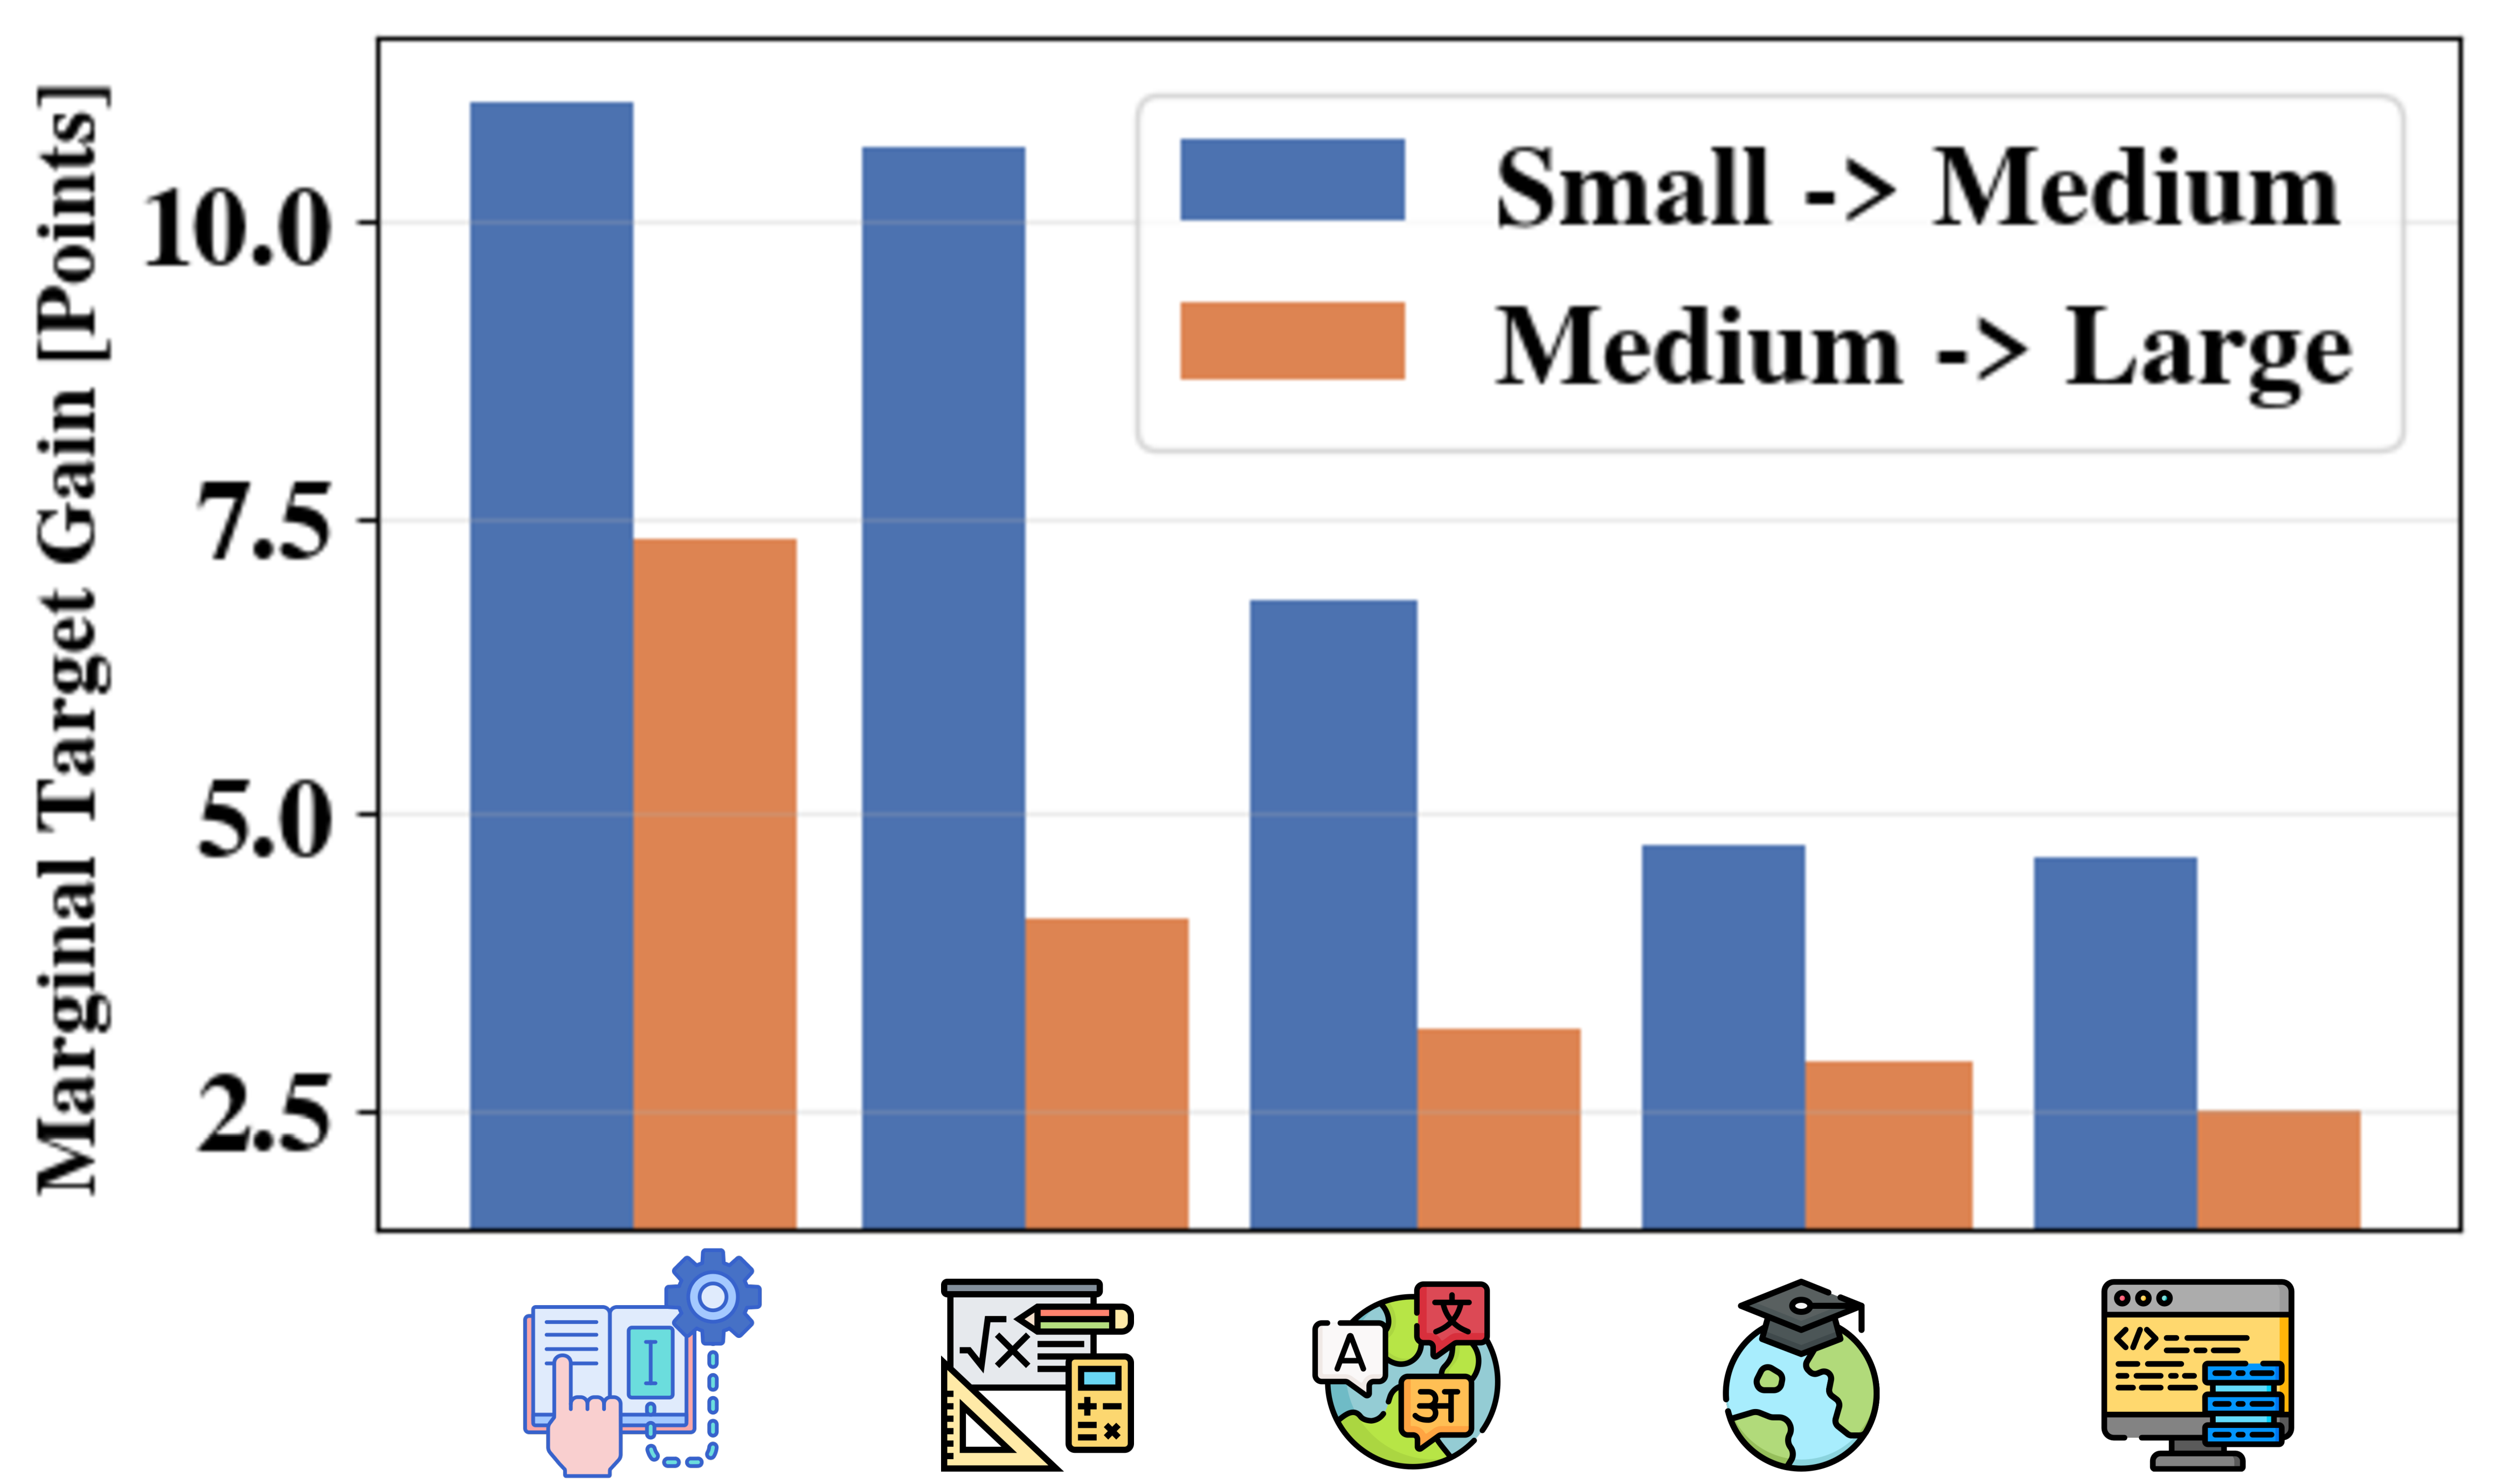
\includegraphics[height=72pt]{figure/Dimenshing.pdf}
    \caption{Diminishing returns}
    \label{fig:diminishing_returns}
  \end{subfigure}\hfill
  \begin{subfigure}[b]{0.270\linewidth}
    \centering
    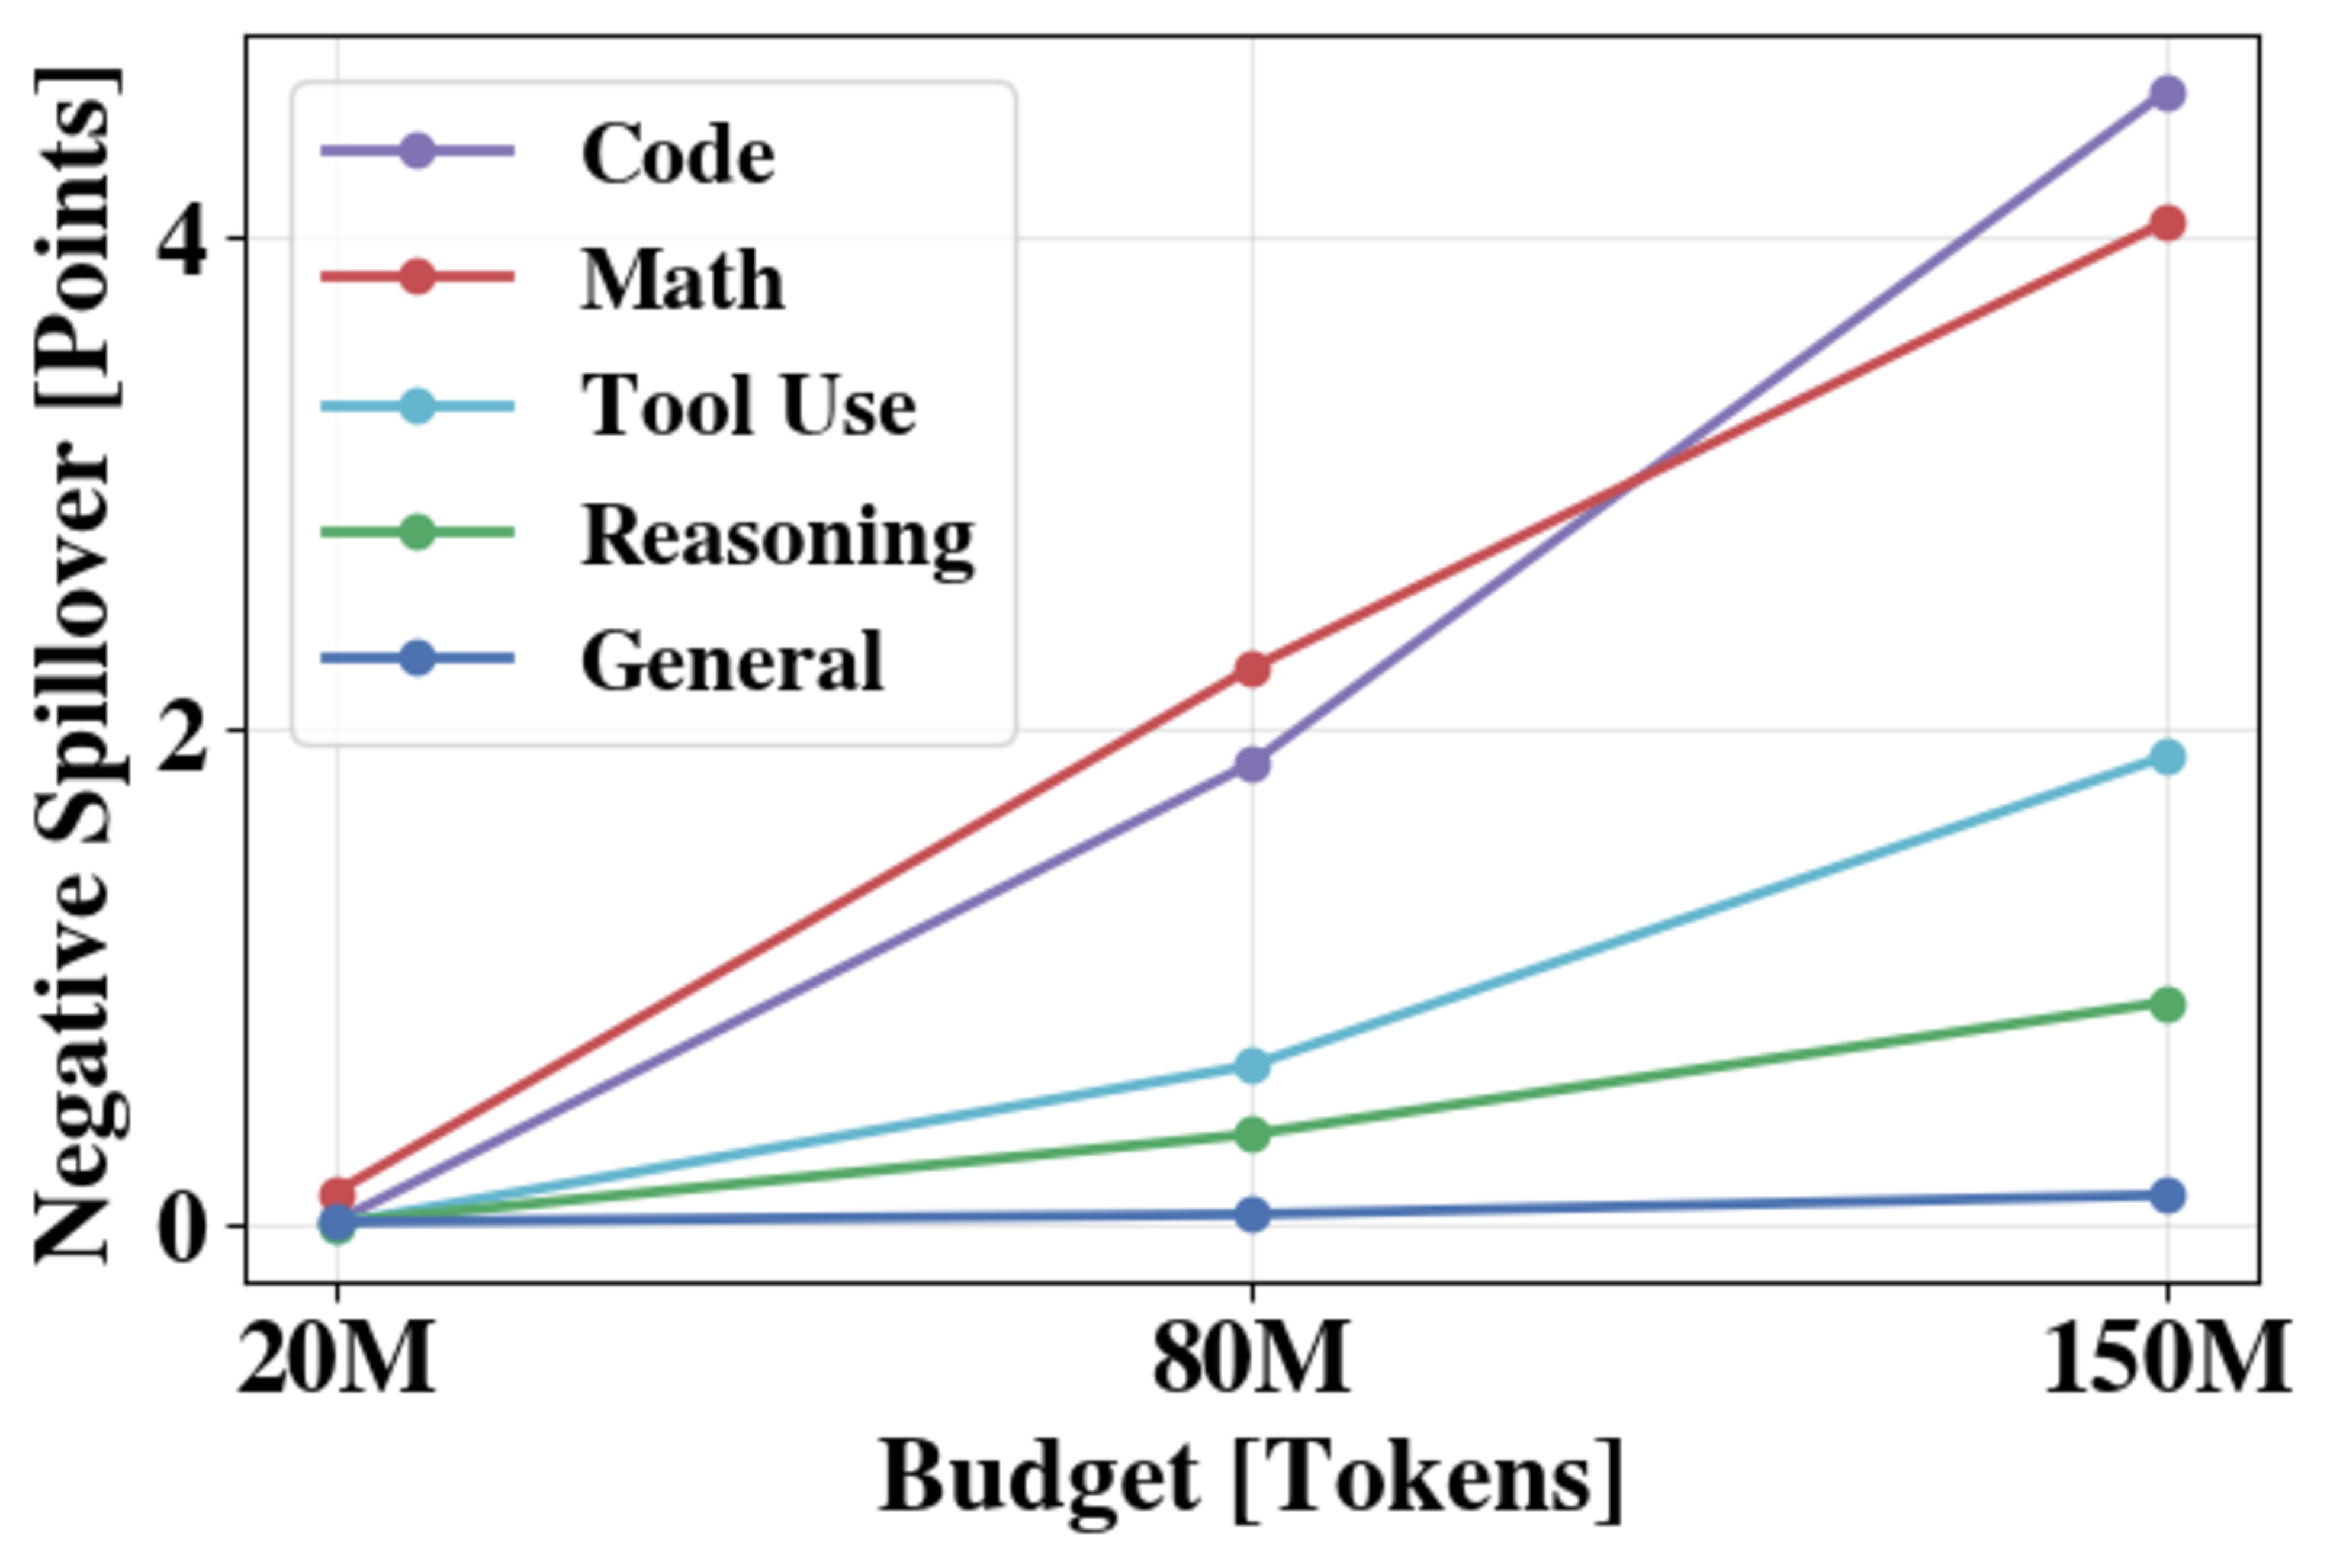
\includegraphics[height=72pt]{figure/spilover.pdf}
    \caption{Rising spillover}
    \label{fig:rising_spillover}
  \end{subfigure}
  \caption{\rev{Exploratory study. (a--b) Cross-capability transfer under
  single-capability distillation: larger budgets sharpen target gains but expose
  stronger negative transfer. (c--d) Budget waste: extra tokens yield smaller
  target gains while increasing harmful spillover to non-target capabilities.}}
  \label{fig:capability_transfer_heatmaps}
  \label{fig:budget_waste_mechanism}
  \vspace{-0.6em}
\end{figure}

\textbf{Observation 1: Distilling a specific capability redistributes performance across other capabilities in a budget-dependent manner.}
\rev{Figure~\ref{fig:capability_transfer_heatmaps}(a--b) shows the transfer
matrices at a small and a large budget. The off-diagonal mass is consistently
non-zero, so optimizing one capability moves the others rather than leaving
them unchanged, and the structure is budget-dependent: at small budgets the
changes are weak and diffuse, whereas at large budgets the diagonal sharpens and
negative off-diagonals appear for specific non-targets.}

\textbf{Observation 2: Capability distillation exhibits substantial budget waste
due to diminishing returns and negative spillover.}
\rev{For the strongest-improving targets, the marginal target gain of
20M$\rightarrow$80M is consistently larger than that of 80M$\rightarrow$150M
(\emph{diminishing returns}, Figure~\ref{fig:diminishing_returns}), while the
drop on non-target capabilities grows with the target's budget (\emph{negative
spillover}, Figure~\ref{fig:rising_spillover}). Beyond a capability-specific
knee point, extra tokens thus buy little target benefit and amplify
cross-capability degradation. Neither effect is new in isolation: off-target
drops are a form of catastrophic
forgetting~\citep{kirkpatrick2017overcoming,luo2023empirical}, and saturation
is ordinary diminishing returns. What allocation can exploit is their
\emph{structure}: transfer is signed, source-specific, and budget-dependent, so
a token's marginal value depends on where the budget has already gone.}

\rev{Effective distillation under a fixed budget must therefore reason jointly
about task-relevant capabilities, their interactions, and allocation. We
formalize this as a sequential budget allocation problem across interdependent capabilities, as follows:}

\begin{problem}[Budget allocation for interdependent capability distillation]\label{prob:budget_alloc}
Given a teacher model \( T \), an initial student model \( S_0 \), a downstream
task \( \tau \), and a total distillation budget \( B \), consider a sequential
distillation process over steps \( t=1,\ldots,T \) with cumulative cost not
exceeding \( B \). At each step \( t \), a capability allocation vector
\( \mathbf{w}_t\in\Delta_{|\mathcal{C}|} \) is selected and applied to update
the student, yielding \( S_t \). Let \( U_\tau(\cdot) \) \rev{be} the task-dependent utility function\rev{;} our target is to determine an allocation policy
\( \{\mathbf{w}_t\}_{t=1}^T \) that maximizes the performance of
the final student model:
\begin{equation}
\max_{\{\mathbf{w}_t\}_{t=1}^T}\ U_\tau\!\left(S_T\right), \
\text{s.t.}\;
\sum_{t=1}^T \mathrm{cost}\!\left(S_{t-1}\!\rightarrow\!S_t\right)\le B
\end{equation}
\end{problem}
